\chapter{Konzept, Entwurf und Implementierung}
\label{cha:implementierung}

% Abschnitt: Implementierungsdetails
\section{Implementierungsdetails}
\label{sec:implementierung:implementierungsdetails}

Wir erklären in diesem Kapitel die einzelnen Funktionen unserer Anwendung ausführlicher. Dies wird unterstützt durch Screenshots und den zugehörigen Mockups, die zu Beginn des Projekts erstellt wurden, um dem Kunden seine Vorstellungen visuell präsentieren zu können.

%Bildervorlage
\begin{figure}[h]
    \centering
    \begin{minipage}{0.49\textwidth}
        \centering
        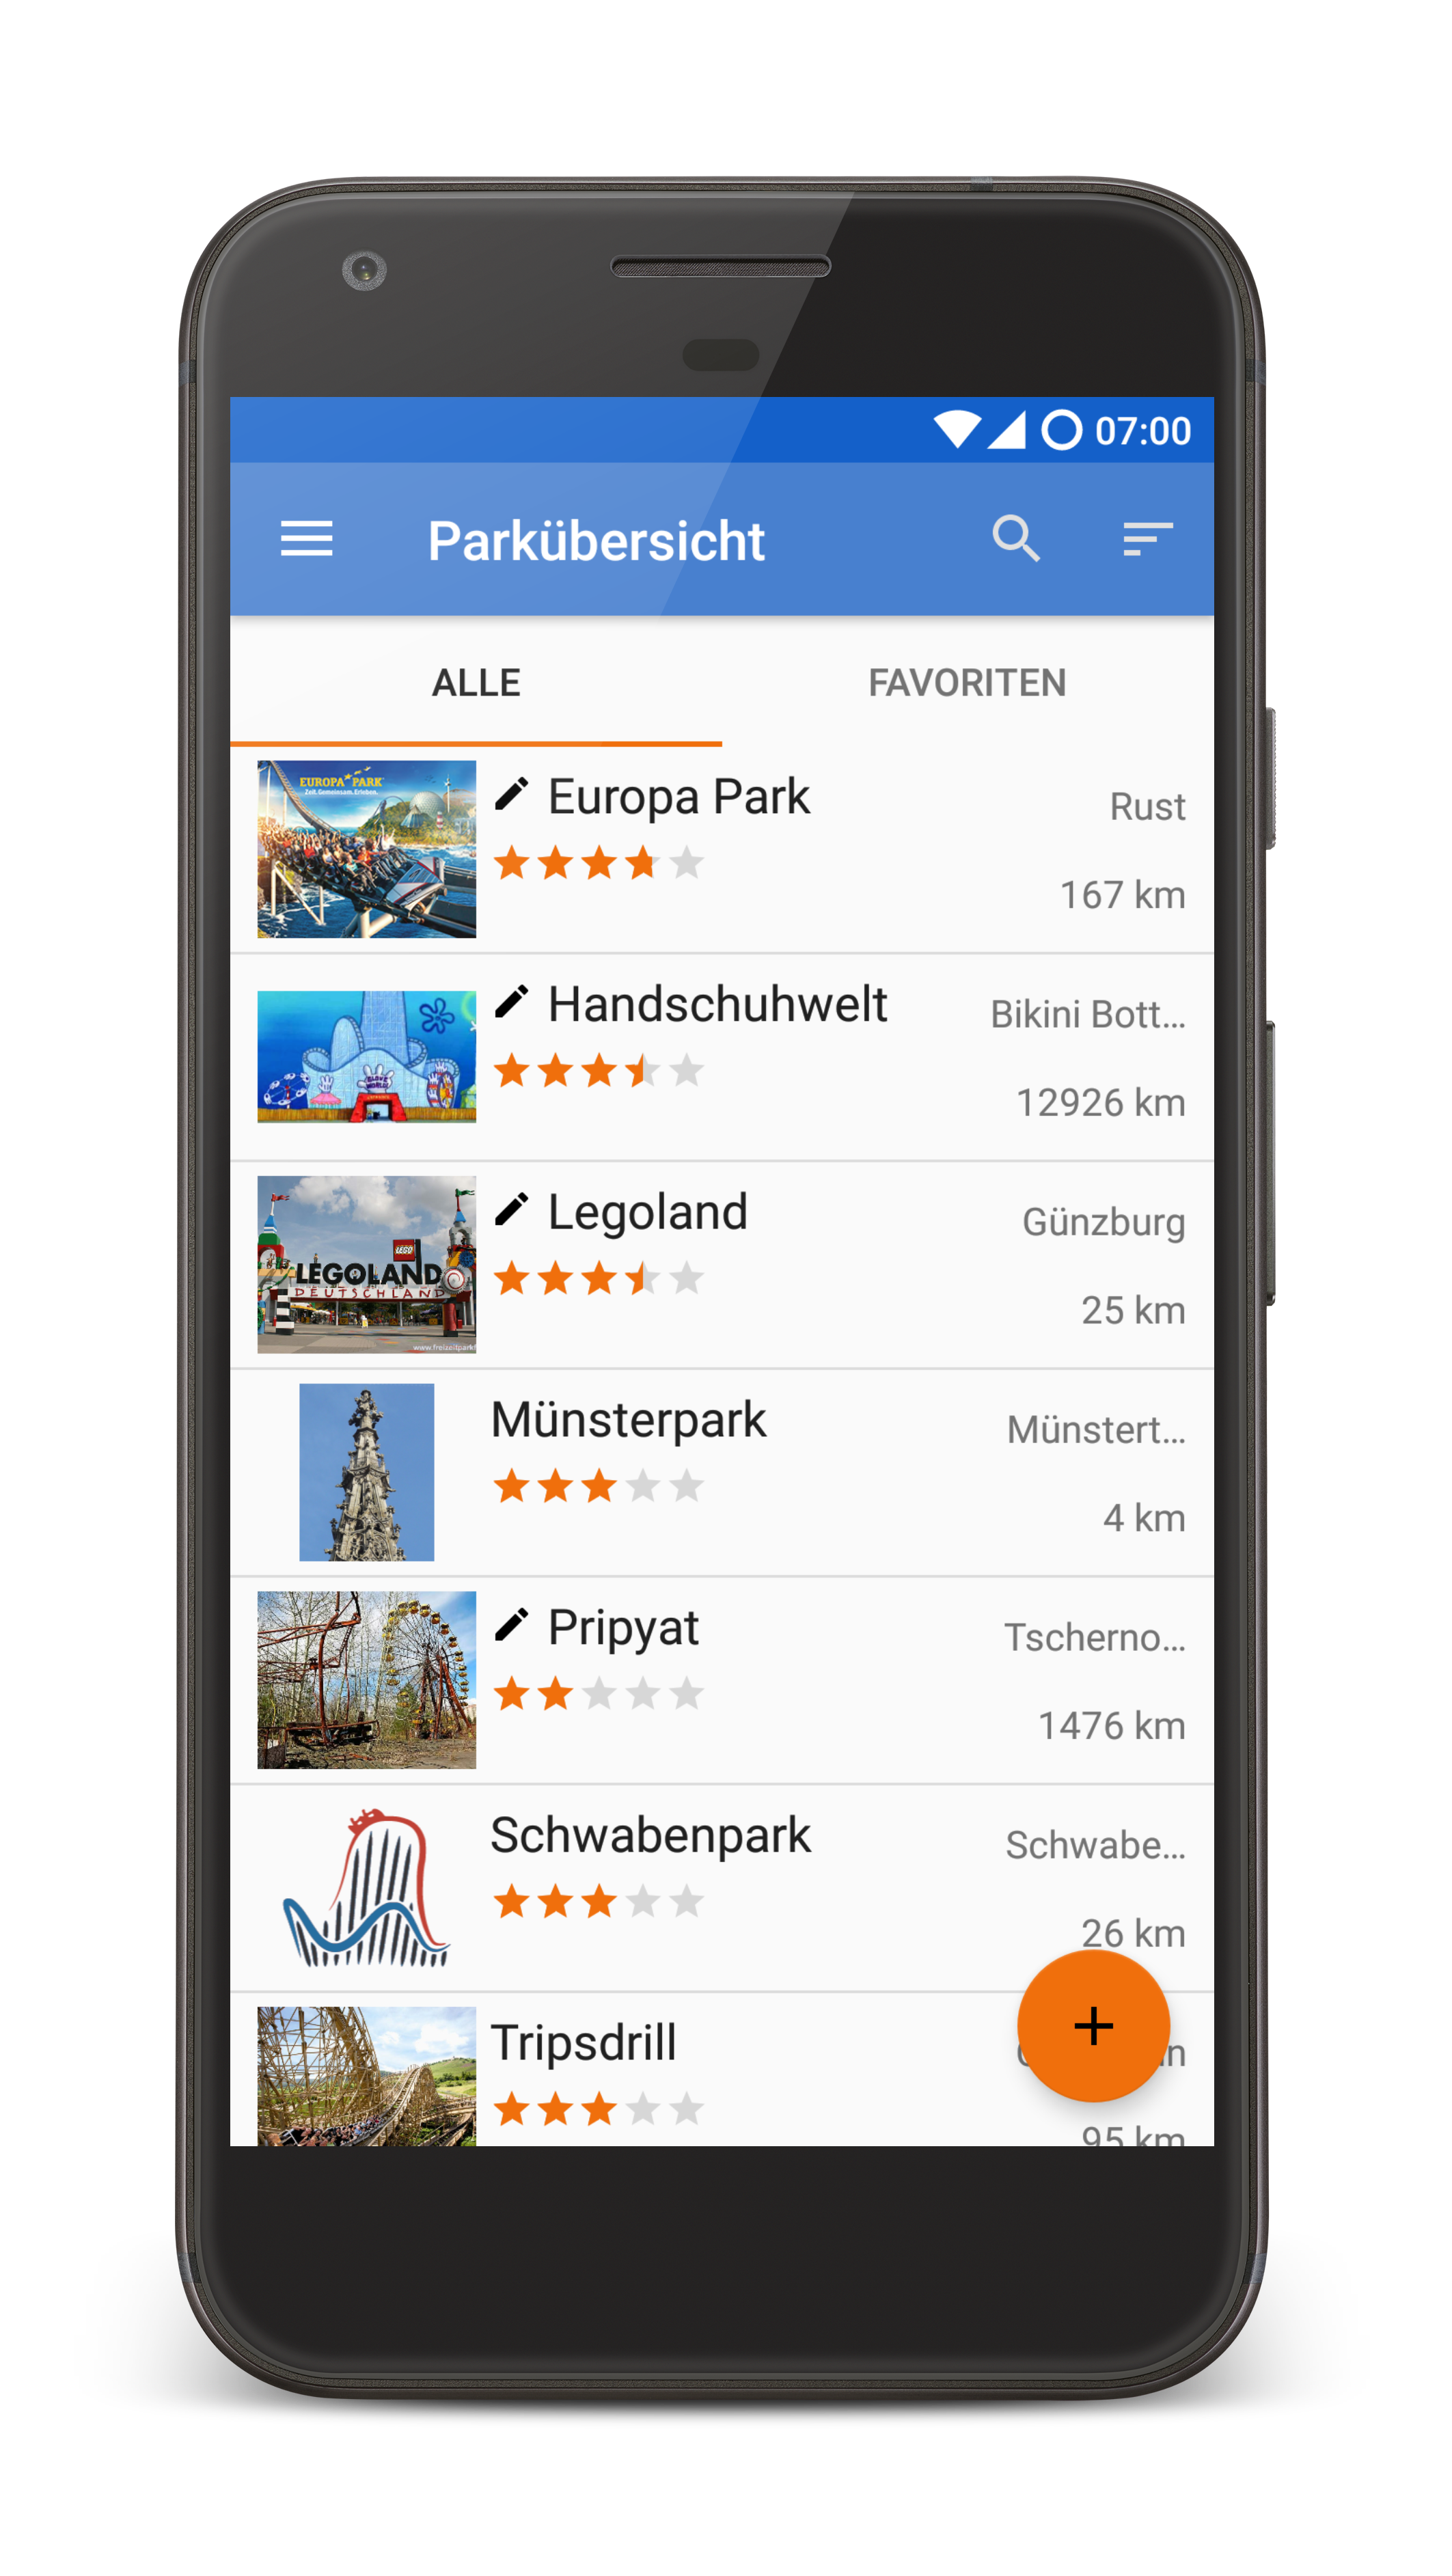
\includegraphics[width=0.49\textwidth]{img/screenshots/ss_parkuebersicht.png}
        \caption{Parkübersicht}
		\label{figure:implementierungparkuebersicht}
    \end{minipage}
    \begin{minipage}{0.49\textwidth}
        \centering
        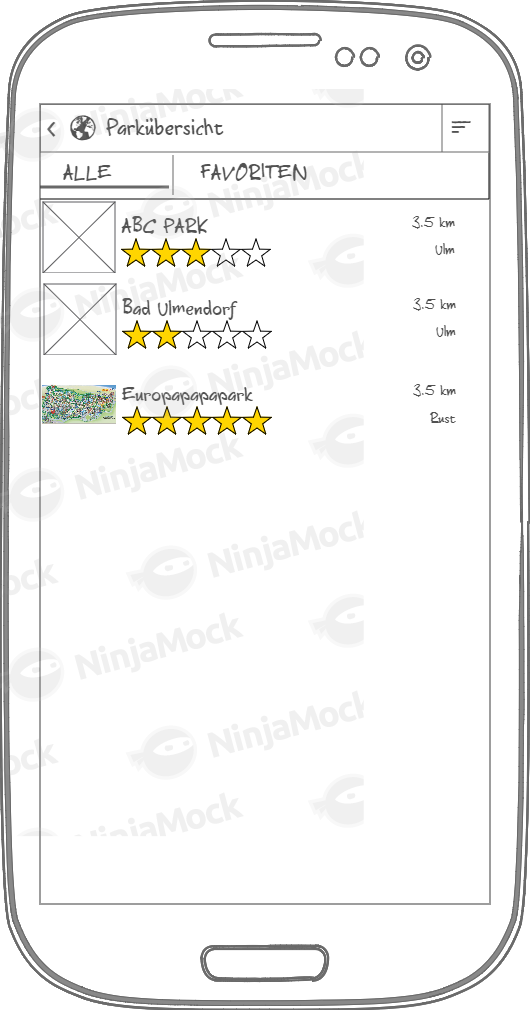
\includegraphics[width=0.49\textwidth]{img/mockups/m_parkuebersicht.png}
        \caption{Mockup Parkübersicht}
    \end{minipage}
\end{figure}

Nach dem Öffnen der Anwendung befindet man sich auf der Startseite unserer App. Diese ist auch zugleich die Parkübersicht, welche in Abbildung \ref{figure:implementierungparkuebersicht} zu sehen ist. Die Pakrübersicht ist eine Liste aller Parks, die man durchsuchen und nach Alphabet, Bewertung oder Entfernung sortieren kann. Außerdem ist die Liste in zwei Tabs unterteilt. Zum Einen das Tab 'Alle', in dem, wie der Name schon sagt, alle Parks angezeigt werden, und als zweites noch das Tab 'Favoriten' in dem alle Parks angezeigt werden, die der Nutzer sich als Favorit markiert hat. 

TODO Bild von der grünen Menüleiste in der man sich einloggen kann

Ist ein Nutzer eingeloggt kann er Park und Attraktionen erstellen und bearbeiten, Wartezeiten eintragen und Bewertungen abgeben. Möchte man sich nicht einloggen kann man die App trotzdem als Informationsquelle nutzen, denn man kann alle Infos wie Wartezeiten und Bewertungen sehen, aber eben nicht selber eintragen. 

Falls man als Nutzer, über den orangenen Plus-Button unten rechts in der Parkübersicht, einen Park erstellt hat, wird neben dem Namen des Parks das Piktogramm eines Stifts angezeigt, was bedeutet, dass man selber Admin des Parks ist und diesen und seine Attraktionen bearbeiten kann. \\

\begin{figure}[h]
    \centering
    \begin{minipage}{0.49\textwidth}
        \centering
        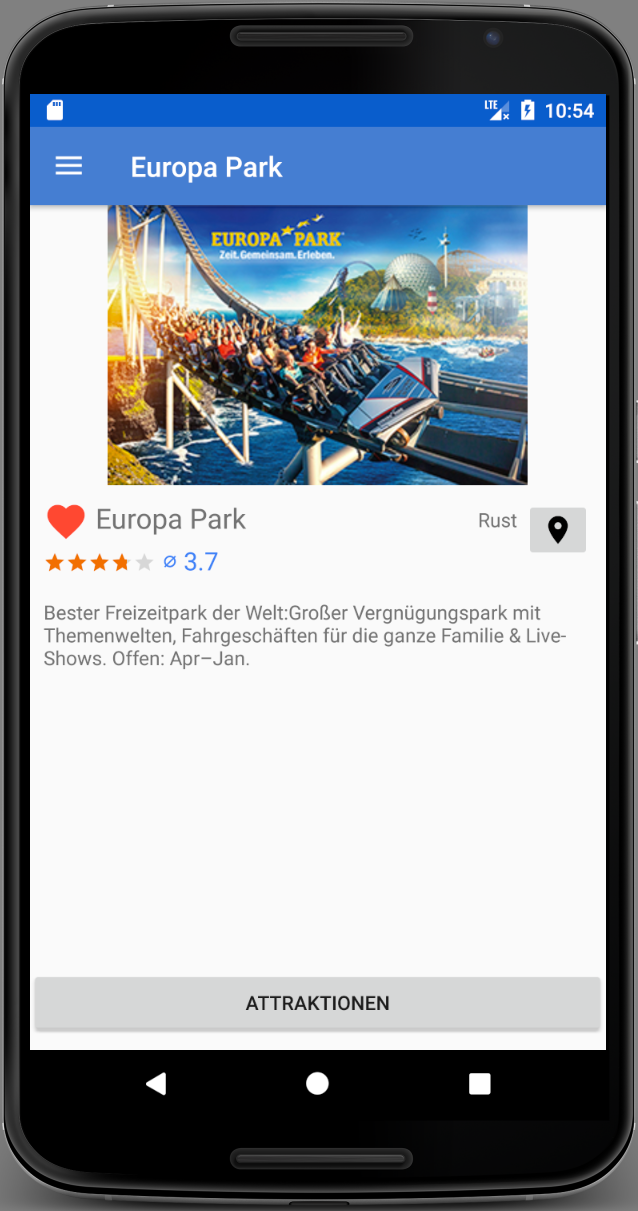
\includegraphics[width=0.49\textwidth]{img/screenshots/ss_parkdetail.png}
        \caption{Parkansicht}
		\label{figure:implementierungparkansicht}
    \end{minipage}
    \begin{minipage}{0.49\textwidth}
        \centering
        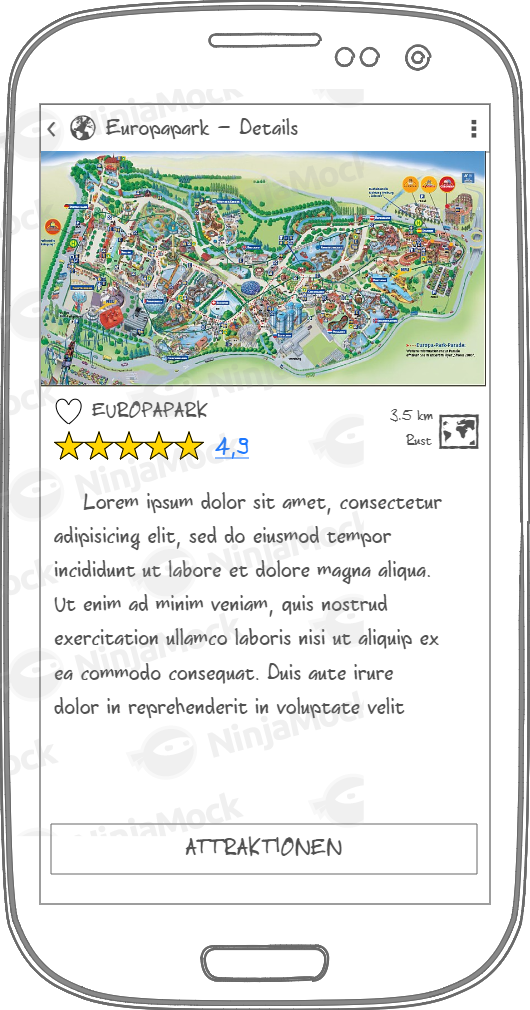
\includegraphics[width=0.49\textwidth]{img/mockups/m_park_detail.png}
        \caption{Mockup Parkansicht}
    \end{minipage}
\end{figure}

Wählt man nun, durch das Tippen auf einen Park, diesen aus, so kommt man als nächstes auf die Parkdetail Seite, welche in Abbildung \ref{figure:implementierungparkansicht} zu sehen ist. 

Oben auf der Seite ist immer ein Bild des Parks zu sehen. Darunter befinden sich das Herz als Symbol für 'Favorit' das sich aktivieren und deaktivieren lässt, der Parkname, der Ort und falls GPS aktiviert ist auch die aktuelle Entfernung zum Park. Der Standort des Parks lässt sich außerdem durch den Button auf der rechten Seite auf GoogleMaps anzeigen. 

Es befindet sich des Weiteren auch noch eine Anzeige der durchschnittlichen Bewertung (Skala von 0 bis 5) auf dieser Seite. Der Durchschnitt wird einmal als Sterne dargestellt und einmal als Dezimalzahl mit einer Nachkommastelle. Durch das Tippen auf die Sterne oder die Zahl lässt sich die Seite der Bewertungen öffnen, was aber weiter unten gezeigt wird. 

Zusätzlich sind auch noch allgemeine Infos zum Park gegeben, wie z. B. die Öffnungszeiten. 

Durch den am unteren Bildrand gelegenen Button 'Attraktionen' kommt man dann weiter zu den Attraktionen des Parks, die wieder, wie auch schon die Parks, als Liste gegeben sind.

\begin{figure}[h]
    \centering
    \begin{minipage}{0.49\textwidth}
        \centering
        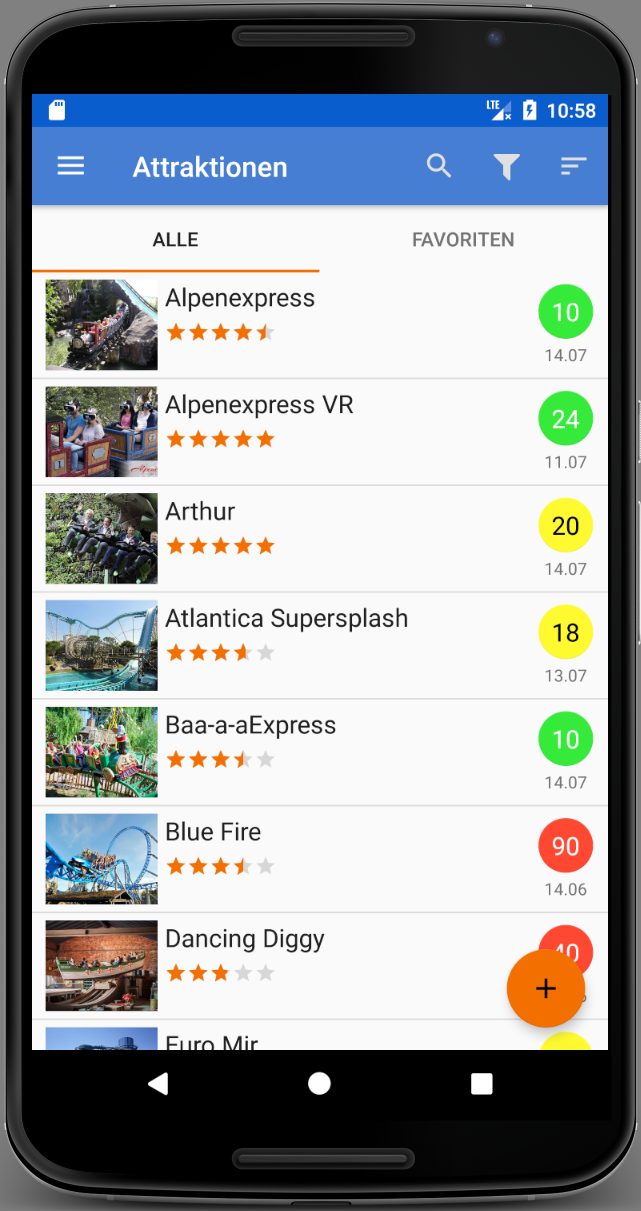
\includegraphics[width=0.49\textwidth]{img/screenshots/ss_attraktionsuebersicht.png}
        \caption{Attraktionsübersicht}
		\label{figure:implementierungattraktionsuebersicht}
    \end{minipage}
    \begin{minipage}{0.49\textwidth}
        \centering
        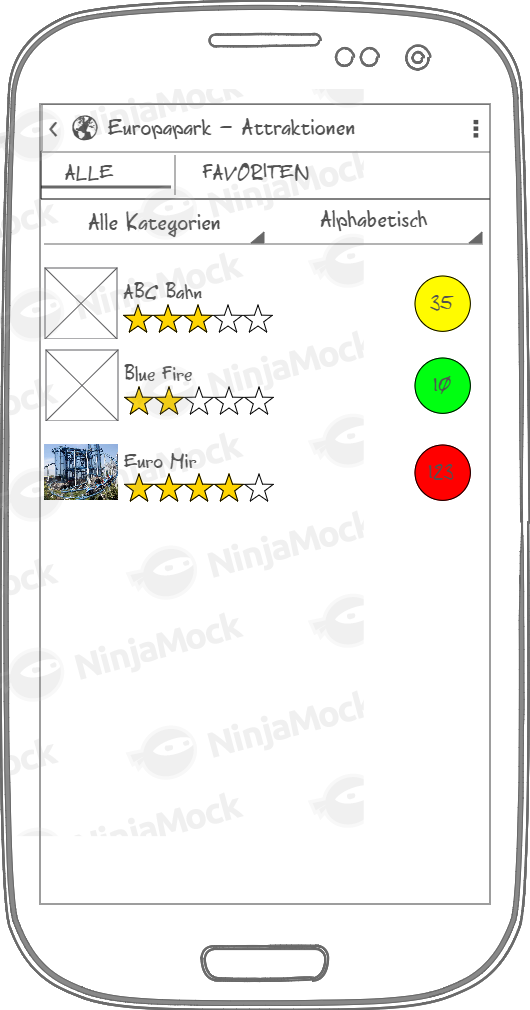
\includegraphics[width=0.49\textwidth]{img/mockups/m_attraktionsuebersicht.png}
        \caption{Mockup Attraktionsübersicht}
    \end{minipage}
\end{figure}

Die Seite aller Attraktionen eines Parks, die sog. Attraktionsübersicht, die in Abbildung \ref{figure:implementierungattraktionsuebersicht} zu sehen ist, ist sehr ähnlich aufgebaut wie die Parkübersicht. Es gibt ebenfalls die Möglichkeiten zur Ansicht aller Attraktionen oder nur der Favoriten und zur Sortierung und Suche, aber hinzu kommt noch die Möglichkeit zum Filtern der Liste nach Kategorien der Attraktionen, wie z. B. Achterbahn oder Essensstand. Die einzelnen Elemente der Liste bestehen aus Bild, Name und Bewertung und dazuhin noch der Wartezeit in Minuten und wann diese eingetragen wurde. Die Farben der Wartezeiten bedeuten einfach dass man entweder nur kurz anstehen muss (grün), durchschnittlich lang (gelb) oder dass momentan die Wartezeit sehr hoch ist (rot). Später wird aber noch genauer auf die Wartezeiten eingegangen und auch der Algorithmus dahinter erklärt. 

\begin{figure}[h]
    \centering
    \begin{minipage}{0.49\textwidth}
        \centering
        
\includegraphics[width=0.49\textwidth]{img/general/todo.jpg}
        \caption{Attraktionsdetail}
		\label{figure:implementierungattraktionsansicht}
    \end{minipage}
    \begin{minipage}{0.49\textwidth}
        \centering
        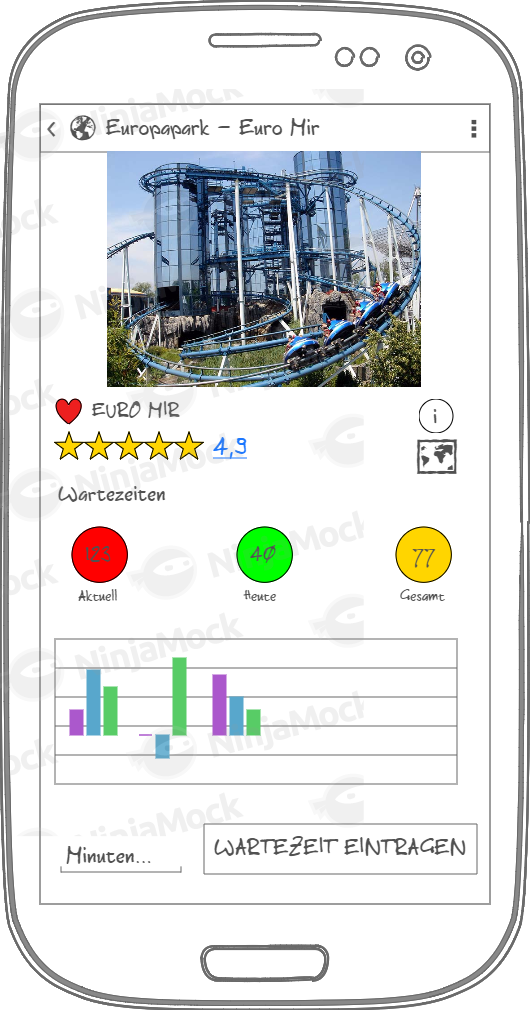
\includegraphics[width=0.49\textwidth]{img/mockups/m_attraktionsdetail.png}
        \caption{Mockup Attraktionsdetail}
    \end{minipage}
\end{figure}

Wählt man nun eine Attraktion aus der Liste aus kommt man zur Detailansicht dieser Attraktion, wie in Abbildung \ref{figure:implementierungattraktionsansicht} zu sehen. 

Auf dieser Seite kann man sich, gleich wie bei Parks, die Attraktion als Favorit hinzufügen, den Standort anzeigen lassen und die Bewertungen ansehen. Neu hinzu kommt, dass man sich noch weitere Informationen über einen 'i'-Button anzeigen lassen kann, wo auch unter Anderem zu sehen ist, in welche der Kategorien die Attraktion gehört. 

Des Weiteren werden hier noch mehr Wartezeiten angezeigt, nämlich links der Durchschnitt der letzten drei Eintragungen, in der Mitte der Tagesdurchschnitt und auf der rechten Seite der Gesamtdurchschnitt. 
Darunter wird eine andere Wartezeitstatistik angezeigt. Hier sind auf der x-Achse die Stunden dargestellt und auf der y-Achse die Minuten. Die Säulen des Diagramms sind dann also die durchschnittliche Wartezeit in der angegebenen Stunde, die aus allen bisher eingetragenen Wartezeiten berechnet wird. 

Ganz unten wird, falls der Nutzer eingeloggt ist, noch ein Feld zum selbst Wartezeiten eintragen angezeigt. Das Eintragen ist aber nur möglich, falls sich der Nutzer zusätzlich noch im Park befindet (Standort muss < 2km vom Park entfernt sein) und nicht schon innerhalb der letzten Stunde für diese Attraktion eine Wartezeit eingetragen hat. 

\begin{figure}[h]
    \centering
    \begin{minipage}{0.49\textwidth}
        \centering
        
\includegraphics[width=0.49\textwidth]{img/general/todo.jpg}
        \caption{Bewertungen}
		\label{figure:implementierungbewertungen}
    \end{minipage}
    \begin{minipage}{0.49\textwidth}
        \centering
        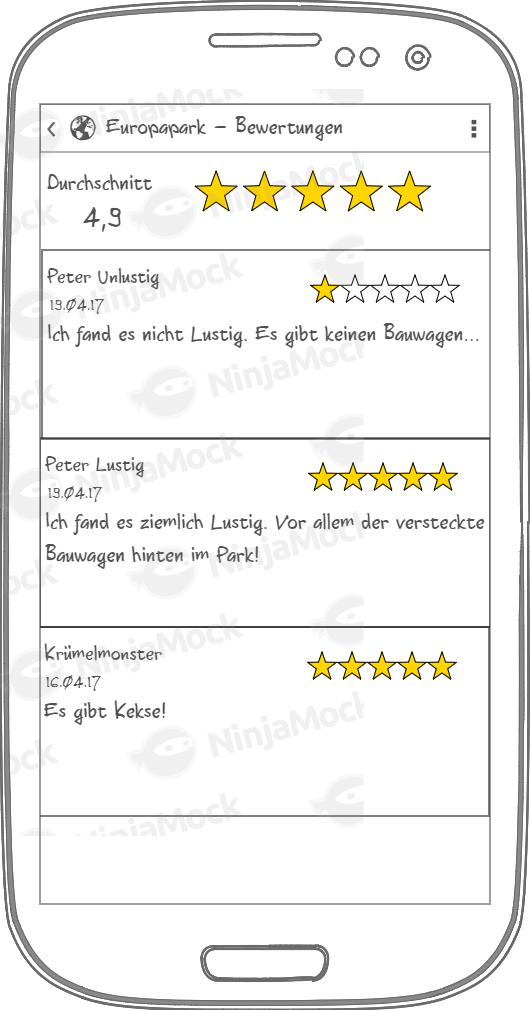
\includegraphics[width=0.49\textwidth]{img/mockups/m_park_bewertungen.png}
        \caption{Mockup Bewertungen}
    \end{minipage}
\end{figure}

Will man nun die Bewertungen einer Attraktion bzw. eines Parks sehen oder diese auch selbst bewerten, kommt man auf die in Abbildung \ref{figure:implementierungbewertungen} zu sehende Activity. 

Ganz oben wird noch einmal der Durchschnitt aller Bewertungen angezeigt. Darunter sind alle bisherigen Bewertungen mit Nutzername, Datum und Kommentar zu sehen.

\begin{figure}[h]
    \centering
    \begin{minipage}{0.49\textwidth}
        \centering
        
\includegraphics[width=0.49\textwidth]{img/general/todo.jpg}
        \caption{Bewertungen}
		\label{figure:implementierungbewerten}
    \end{minipage}
    \begin{minipage}{0.49\textwidth}
        \centering
        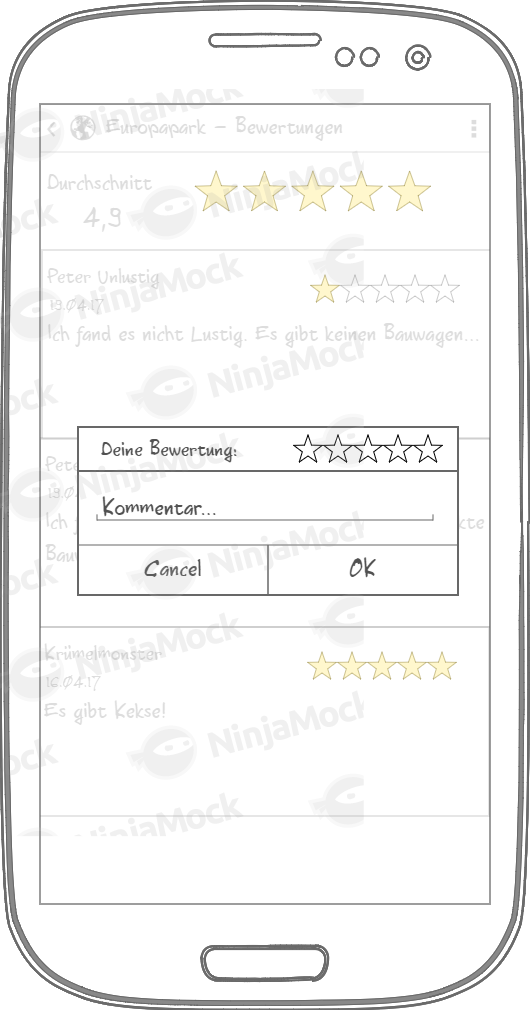
\includegraphics[width=0.49\textwidth]{img/mockups/m_bewertung_verfassen.png}
        \caption{Mockup Bewertung verfassen}
    \end{minipage}
\end{figure}

Um selbst eine Bewertung abzugeben tippt man auf den orangenen Plus-Button unten Rechts und es Öffnet sich ein Eingabedialog, wie in Abbildung \ref{figure:implementierungbewerten} zu sehen. Falls man zu diesem Park bzw. dieser Attraktion eine Bewertung abgegeben hat, so wird diese hier angezeigt und man kann sie bearbeiten, aber es wird keine neue erstellt. Hat man bisher noch nicht bewertet, vergibt man jetzt 0 bis 5 Sterne, schreibt ein Kommentar und speichert dann mit 'OK'.

\begin{figure}[h]
    \centering
    \begin{minipage}{0.49\textwidth}
        \centering
        
\includegraphics[width=0.49\textwidth]{img/general/todo.jpg}
        \caption{Wartezeiten}
		\label{figure:implementierungwartezeiten}
    \end{minipage}
    \begin{minipage}{0.49\textwidth}
        \centering
        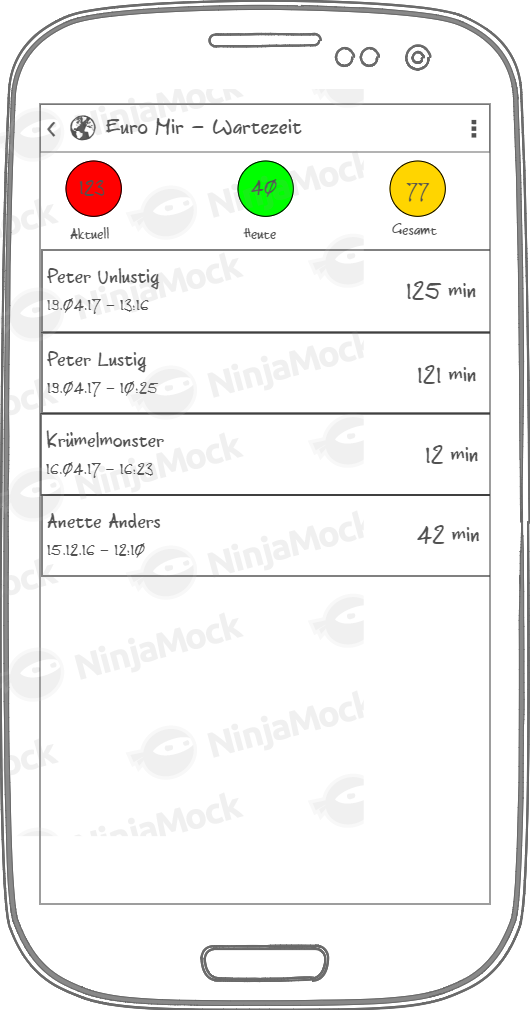
\includegraphics[width=0.49\textwidth]{img/mockups/m_wartezeiten.png}
        \caption{Mockup Wartezeiten}
    \end{minipage}
\end{figure}






















% Abschnitt: Besonderheiten 
\section{Besonderheiten}
\label{sec:implementierung:besonderheiten}

TODO

\subsection{Wartezeit berechung und -darstellung}
\label{sec:implementierung:besonderheiten:wartezeit}

\subsection{Client-Server-Kommunikation mit Azure}
\label{sec:implementierung:besonderheiten:azure}

%Download- und Upload-Verlauf-Modell

\subsection{User-Verwaltung mit Firebase}
\label{sec:implementierung:besonderheiten:firebase}

%Firebase Modell?

\subsection{Parkverwaltung}
\label{sec:implementierung:besonderheiten:parkverwaltung}



% Abschnitt: Architektur
\section{Architektur}
\label{sec:implementierung:architektur}

\subsection{Datenmodell und -speicherung}
\label{sec:implementierung:architektur:datenmodell}

TODO

\subsection{Klassen- und Activity-Architektur}
\label{sec:implementierung:architektur:klassenmodell}

TODO

\subsection{Arbeitsaufteilung}
\label{sec:implementierung:architektur:arbeitsaufteilung}

Während der Implementation wurden die Aufgaben so aufgeteilt, dass jeder aus dem Team immer für eine bestimmte Aufgabe zuständig war und diese durch alle Schichten durch erledigen musste. Bei großen Aufgaben, wie dem Spielablauf, wurden die Aufgabe zudem in kleinere Schritte aufgeteilt. Da die App aus mehreren unabhängigen Bereichen besteht, konnten die Aufgaben gut eingeteilt werden, ohne dass es zu Behinderungen kommt. Wenn gerade keine Arbeit für eine Person angefallen war, beschäftigte diese sich mit Verbesserungen, Testen von Funktionen oder mit der Weiterentwicklung des Designs.

% Abschnitt: Schwierigkeiten während der Implementierung 
\section{Schwierigkeiten während der Implementierung}
\label{sec:implementierung:schwierigkeiten}	

TODO

\begin{itemize} 
\item 1
\item 2
\end{itemize}




